


% Bounded identity
\begin{frame}{\tciii{} Signed distances}

\begin{columns}
\begin{column}{0.45\linewidth}
\begin{block}{Bounded identity function}
\begin{equation}
\alpha: \begin{cases}
& \text{ if } x \geq 1: \alpha(x) = 1\\ 
& \text{ if } x \leq -1: \alpha(x) = -1\\ 
& \text{ else: }  \alpha(x) = x
\end{cases}
\end{equation}
\end{block}
\end{column}

\begin{column}{0.45\linewidth}
\begin{figure}
\centering
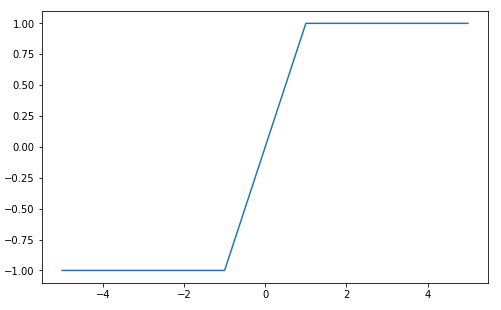
\includegraphics[width=.9\linewidth]{images/GENE/images/bounded.png}
\end{figure}
\end{column}
\end{columns}

\end{frame}


% Final functions
\begin{frame}{\tciii{} Distance functions}

\begin{columns}
\begin{column}{0.60\linewidth}
\begin{block}{pL2-GENE}
\begin{equation}
\alpha \left  ( \prod_{k=1}^D n_1^k - n_2^k \right ) \sqrt{\sum_{j=1}^D \left( n_1^j - n_2^j \right)^2 }
\end{equation}
\end{block}
\end{column}

\begin{column}{0.35\linewidth}
\begin{figure}
\centering
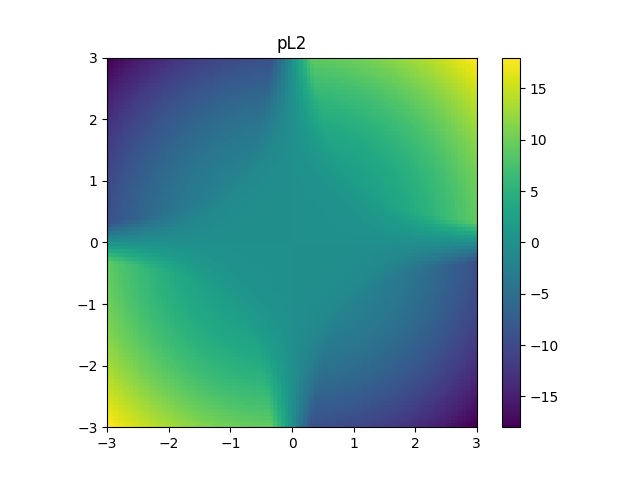
\includegraphics[width=\linewidth]{images/GENE/images/distance_pL2.png}
\end{figure}
\end{column}
\end{columns}

\begin{columns}
\begin{column}{0.60\linewidth}
\begin{block}{tag-GENE}
\begin{equation}
\sum_{j=2}^D \alpha(n_1^j - n_2^1) e^{-|n_1^j - n_2^1|}
\end{equation}
\end{block}
\end{column}

\begin{column}{0.35\linewidth}
\begin{figure}
\centering
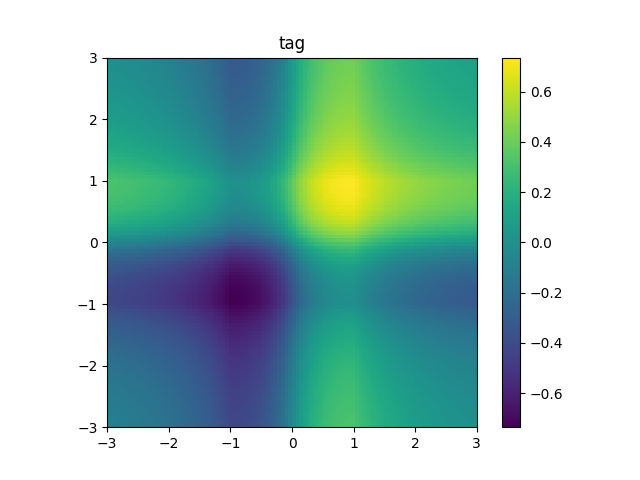
\includegraphics[width=\linewidth]{images/GENE/images/distance_tag.png}
\end{figure}
\end{column}
\end{columns}

\end{frame}


\begin{frame}{\tcv{} Classic Control}%
        \def\figwidth{0.16\linewidth}%
        \def\yleg{Fitness}%
        \begin{textblock*}{2cm}(0cm,0.7cm) % {block width} (coords)
            $\%$noise
        \end{textblock*}
        \begin{table}%[!t]
            \centering
            \begin{tabular}{ccccccc}
                && $0\%$ & $200\%$ & $400\%$ & $600\%$ & $800\%$ \\
                \raisebox{3\normalbaselineskip}[0pt][0pt]{\rotatebox[origin=c]{90}{\cartpole}} &
                \raisebox{3\normalbaselineskip}[1cm][0cm]{\rotatebox[origin=c]{90}{\vspace{1cm}\yleg}}&
                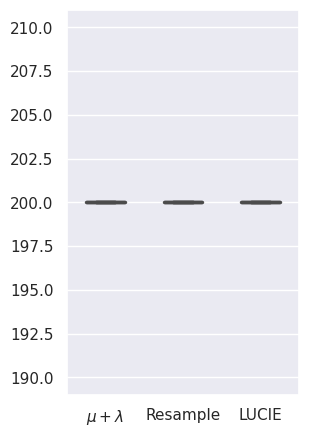
\includegraphics[width=\figwidth]{images/LUCIE/cartpole/boxplot_cartpole_0.png} &
                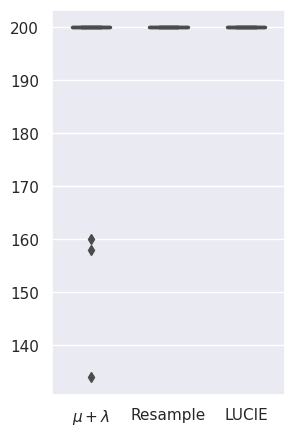
\includegraphics[width=\figwidth]{images/LUCIE/cartpole/boxplot_cartpole_200.png} &
                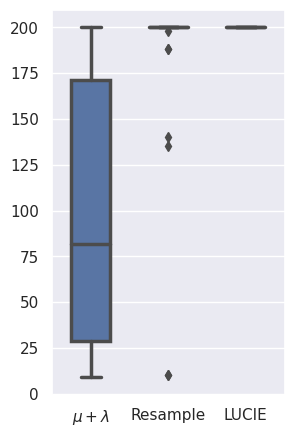
\includegraphics[width=\figwidth]{images/LUCIE/cartpole/boxplot_cartpole_400.png} &
                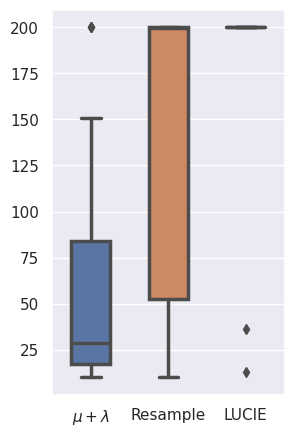
\includegraphics[width=\figwidth]{images/LUCIE/cartpole/boxplot_cartpole_600.png} &
                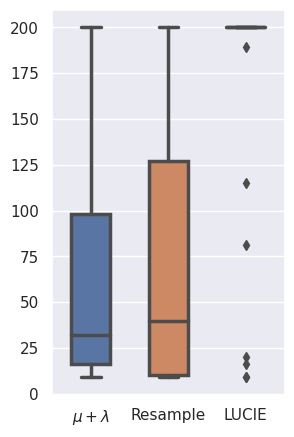
\includegraphics[width=\figwidth]{images/LUCIE/cartpole/boxplot_cartpole_800.png}\\
            \end{tabular}
%				\caption{Final validation fitness for \cartpole{} neuroevolution under posterior uniform noise.}
%				\label{table:cartpole-uniform-eval-validation}
        \end{table}

        \vspace{-1em}

        \def\figwidth{0.16\linewidth}
        \def\yleg{Fitness}
        \begin{table}[]
            \centering
            \begin{tabular}{ccccccc}
%					&& 0\% & 200\% & 400\% & 600\% & 800\% \\
                \raisebox{3.5\normalbaselineskip}[0pt][0pt]{\rotatebox[origin=c]{90}{\acrobot{}}} &
                \raisebox{3.5\normalbaselineskip}[1cm][0cm]{\rotatebox[origin=c]{90}{\vspace{1cm}\yleg}}&
                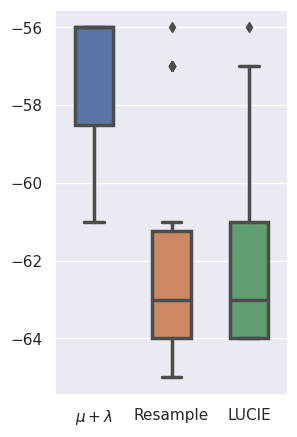
\includegraphics[width=\figwidth]{images/LUCIE/acrobot/boxplot_acrobot_0_u.png} &
                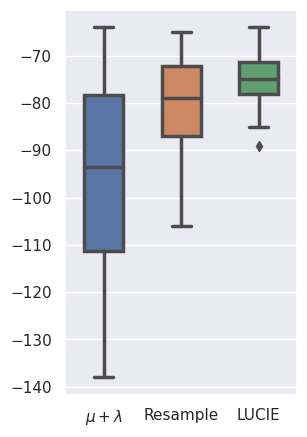
\includegraphics[width=\figwidth]{images/LUCIE/acrobot/boxplot_acrobot_200_u.png} &
                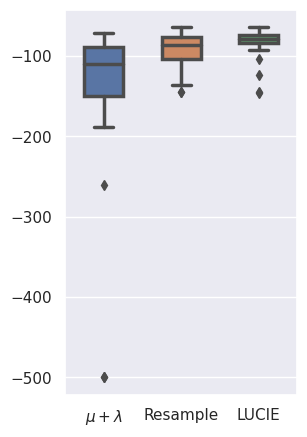
\includegraphics[width=\figwidth]{images/LUCIE/acrobot/boxplot_acrobot_400_u.png} &
                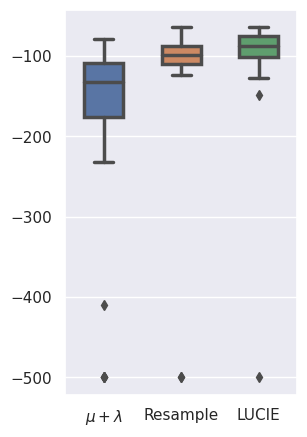
\includegraphics[width=\figwidth]{images/LUCIE/acrobot/boxplot_acrobot_600_u.png} &
                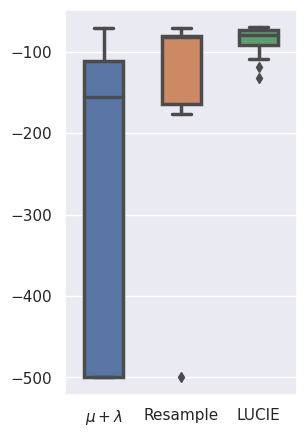
\includegraphics[width=\figwidth]{images/LUCIE/acrobot/boxplot_acrobot_800_u.png}\\
            \end{tabular}
%				\caption{Final validation fitness for Acrobot neuroevolution under posterior uniform noise.}
%				\label{table:acrobot-uniform-eval-validation}
        \end{table}

\end{frame}